\chapter{Majoron Decay Search}
To search for evidence of Majoron decays of $^{130}$Te, which deposit energy in CUORE's detectors with energies ranging up to the 2528 keV Q-value of $^{130}$Te as shown in \autoref{fig:Majoron Spectrum}, a precise understanding of the energy spectrum measured by CUORE is needed.
In essence, this search is purely a comparison of a $H_0$ hypothesis of physics without a Majoron contribution in favor of an $H_1$ hypothesis that includes Majoron decay.
However, constructing a ``true" $H_0$ model is not a trivial task, as it contains over 60 independent components in a background model, all of which are fitted simultaneously.
In the worst-case scenario, an incorrect model could, by pure misfortune, be a good fit to the data; therefore, considerable work is undertaken to properly understand and characterize the components of the background model in CUORE.

\section{Background Sources in CUORE}
As discussed in \autoref{ssec:Parts Selection and Cleaning} and \autoref{ssec:Cryostat_Radiopurity}, there are multiple backgrounds that need to be considered when understanding the energy spectrum measured by the detectors.
These background come from radioactive contaminations in the cryostat components of CUORE and from external sources such as muons.
This process is nearly identical to that used in CUORE-0, where a 57-component fit was performed to describe the energy spectrum observed \cite{Alduino:2016vtd}.
As CUORE-0 utilized a CUORE-like tower with the same cleaning and fabrication, the radioactive sources on the tower structures are expected to be the same in CUORE.
In addition, environmental sources such as muons are expected to be the same as well as CUORE is located in the same underground hall in LNGS as CUORE-0.
However, with the new cryostat used for CUORE, the backgrounds due to the rest of the cryostat will differ from those in CUORE-0.

\subsection*{Source Reconstruction}
To perform a fit to the data, fitting an exhaustive list of every component in CUORE with every possible contamination would be the most straightforward approach.
However, due to the limited statistics in CUORE data\footnote{One of the unfortunate side effects of having a clean detector is that the number of available statistics to disentangle sources and their locations is considerably more difficult.}, many of these sources are virtually indistinguishable from one another, as shown in \autoref{fig:degenerate_sources}.
To solve this issue, these sources with ``degenerate" spectra are combined in the analysis and are combined into the same source in the fit.
\begin{figure}[htbp]
    \centering
    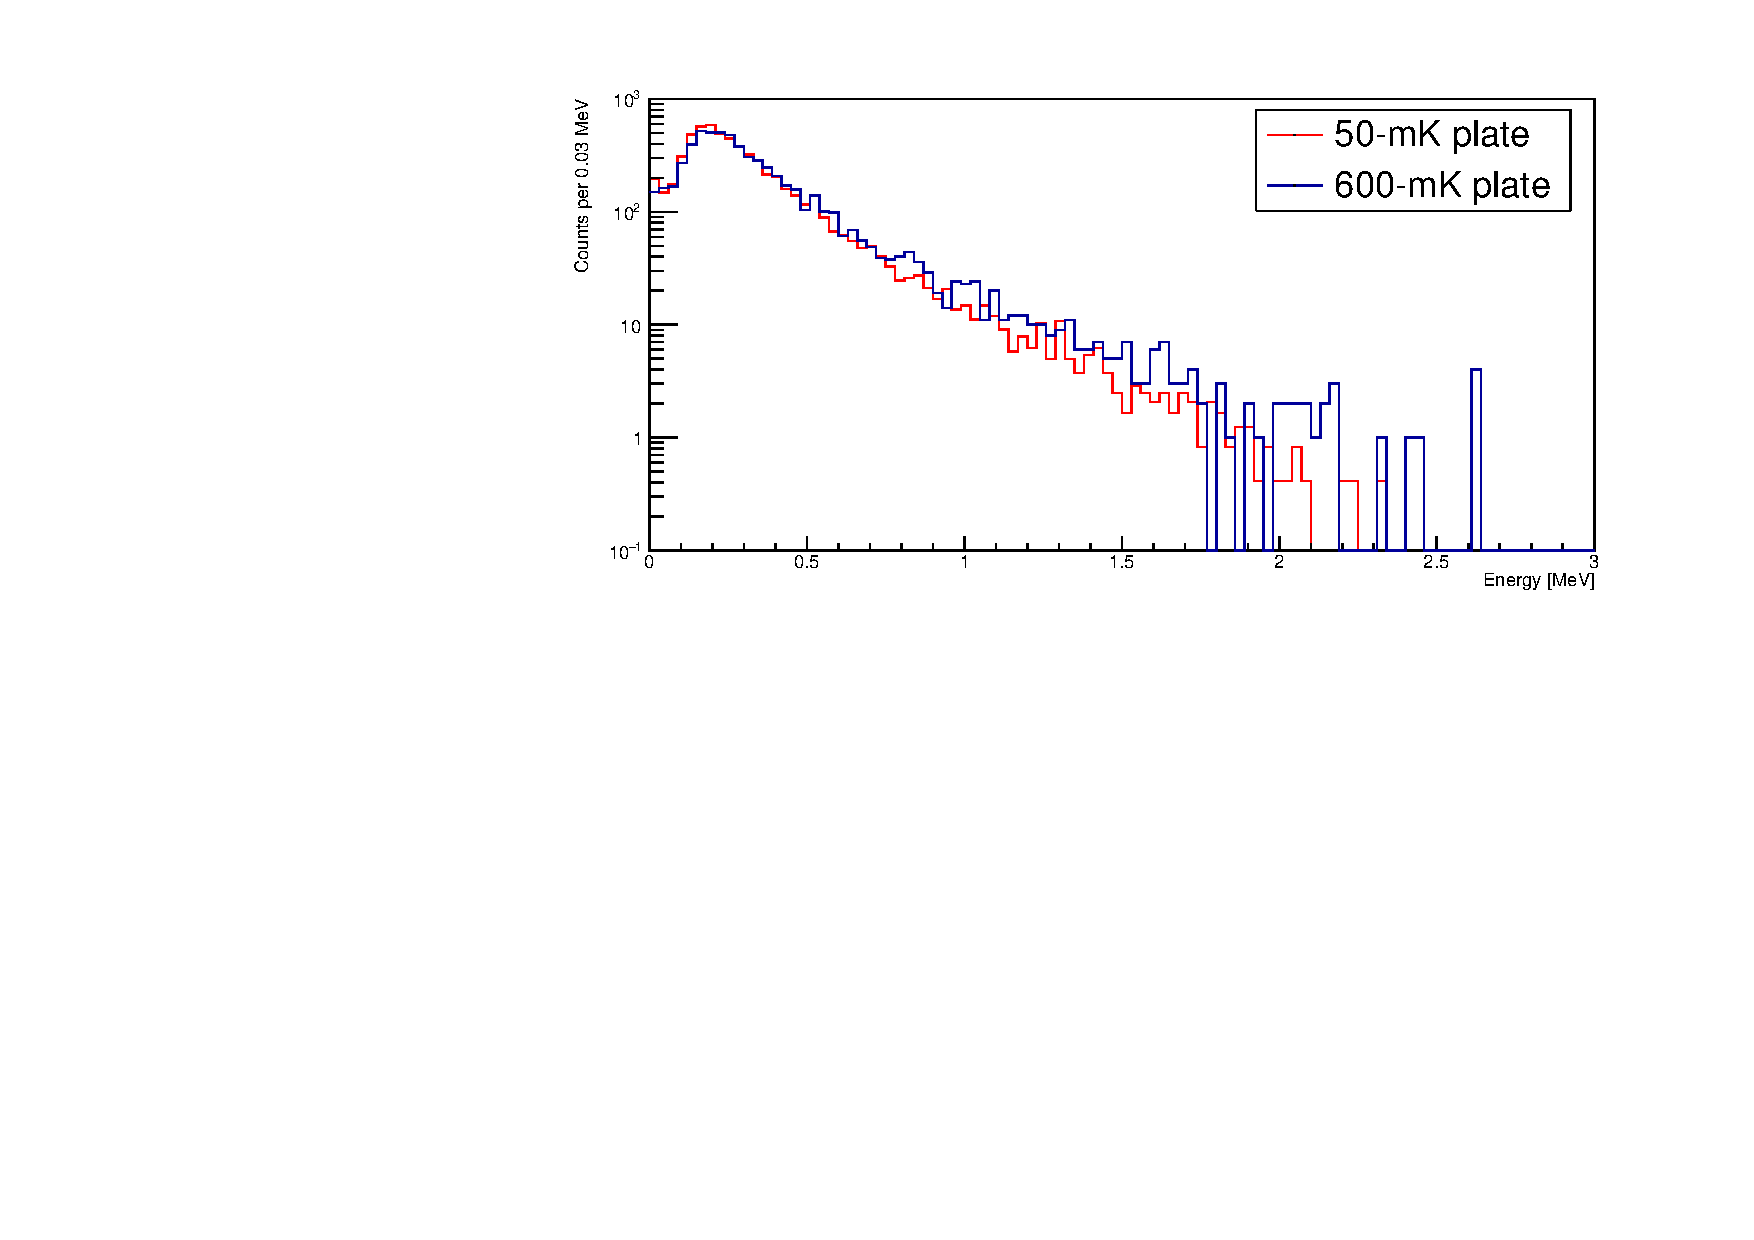
\includegraphics[width=0.8\linewidth]{Figures/th232_copper_plates.pdf}
    \caption[Simulated rates from a $^{232}$Th source on the 50-mK and 600-mK plates.]
    {Simulated rates from a $^{232}$Th source on the 50-mK and 600-mK plates.
    The spectra produced by these two materials are nearly identical and are indistinguishable for performing a fit.}
    \label{fig:degenerate_sources}
\end{figure}
In this way, much of the complexity of the fit can be reduced by combining sources as many cryostat components produce similar energy spectra for various contaminations, particularly for elements such as the copper vessels which are composed of the same material and are expected to have similar contaminations.
While some of this degeneracy could be removed by including the complete position information in the fit, only information on the general position of the incident radiation is included in the fit as the information from $\approx1000$ crystals would add significantly more free parameters, require a similar increase in the computation time to generate simulated spectra for each crystal, and further split the limited statistics by the same factor.

However, this position information for the sources can be a strong indicator for asymmetric sources in the cryostat.
For example, in CUORE-0, an excess of $^{232}$Th and $^{40}$K events on some crystals were determined to be due to spot sources on the 50-mK shield and the bottom of the external lead shield.
While CUORE benefits from improved procedures for handling and cleaning materials, it is not unreasonable to expect that there may be similar situations on CUORE, and indeed, excesses are observed in the data.
A fully complete background model would include these sources, but these geometrical differences are included as a systematic in the fits produced by the data, as data is selected by different geometrical slicings of the data, e.g. by fitting only odd/even floors or by odd/even towers.

\begin{figure}
    \centering
    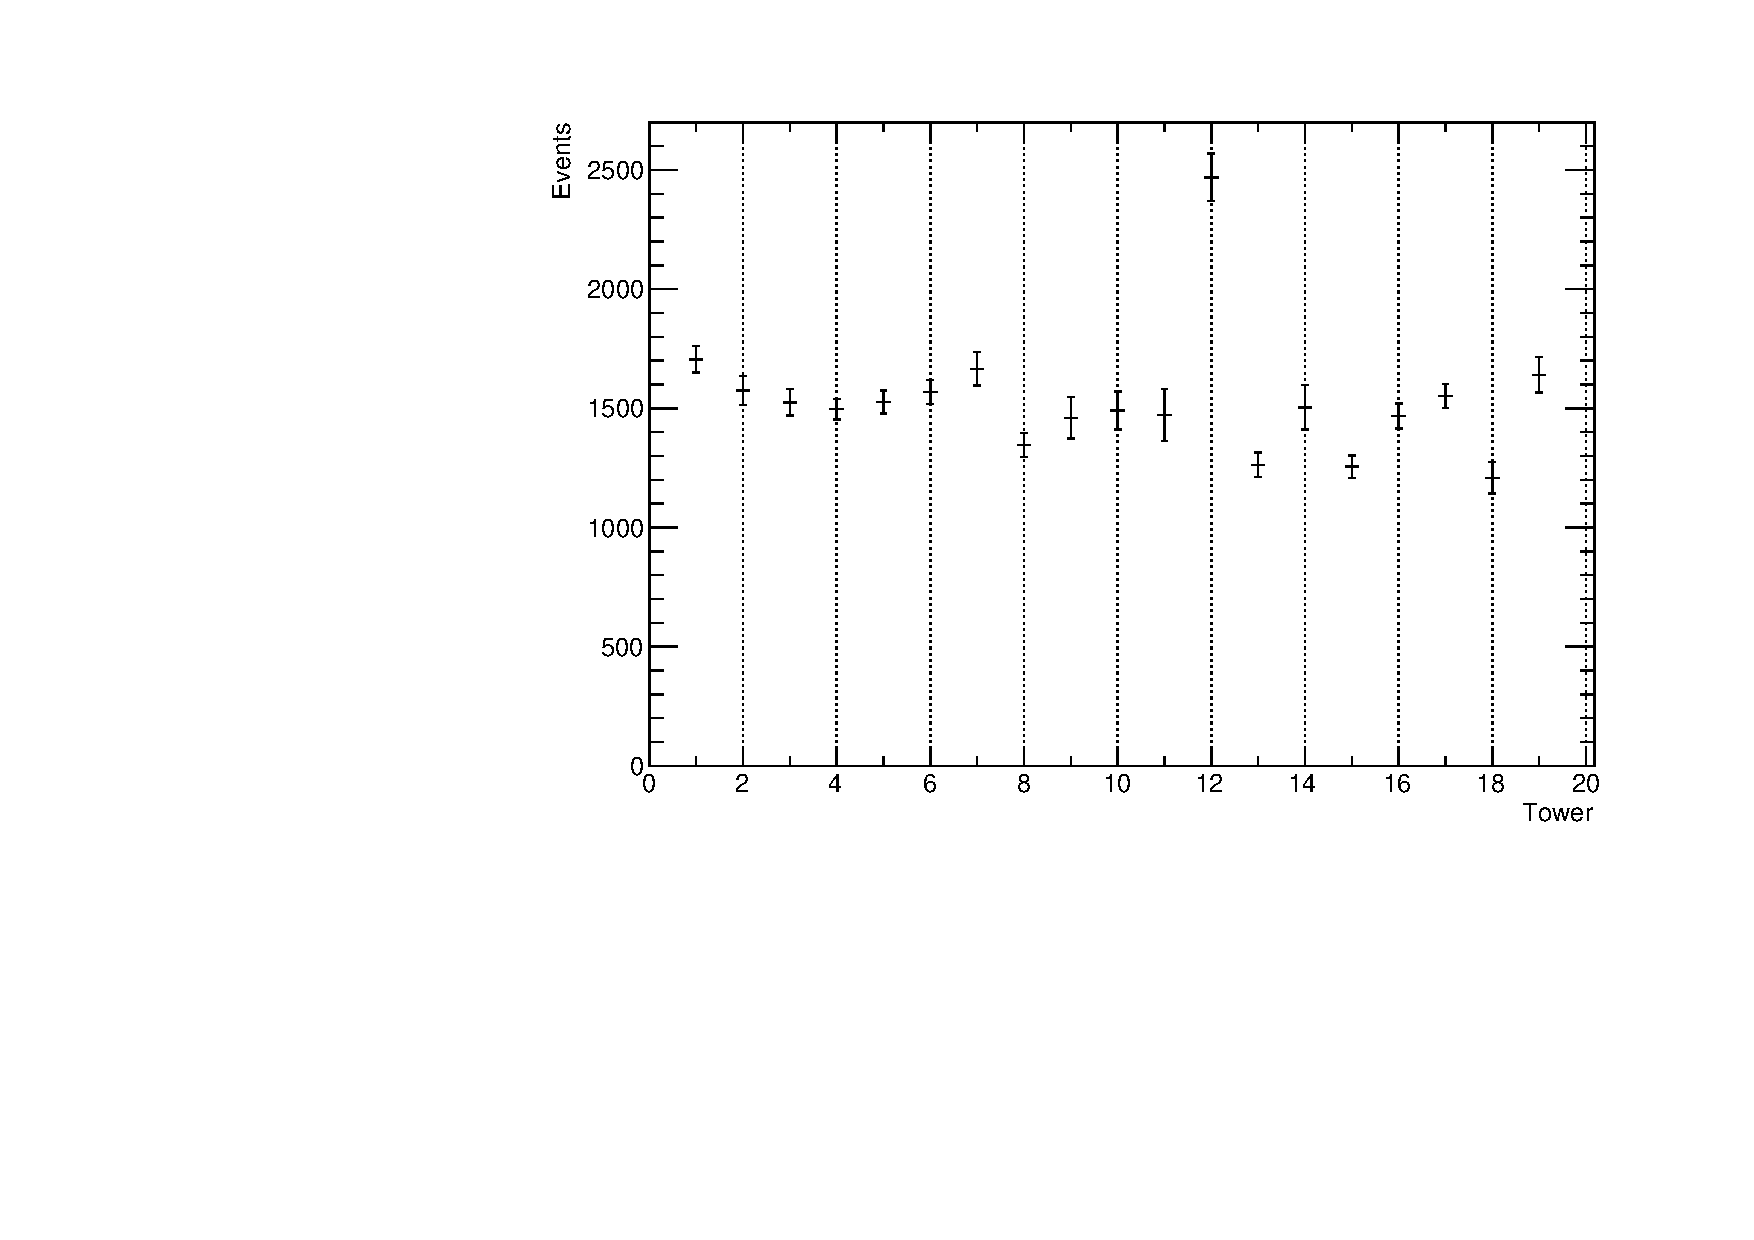
\includegraphics[width=0.8\linewidth]{Figures/k40ByTower.pdf}
    \caption[The number of $^{40}$K events at  on each CUORE tower.]
    {The number of $^{40}$K events on each CUORE tower.
    Tower 12 has considerably more $^40$K than the others.}
    \label{fig:my_label}
\end{figure}
include figures for search for spot-sources on the towers.



\section{Markov Chain Monte Carlo}
\label{sec:MCMC}
Performing a simultaneous fit of $60+$ spectra is a non-trivial challenge, particularly as each component to the fit is comprised of a 


The method used for performing this fit to the data is Markov Chain Monte Carlo (MCMC).
This method can be thought of as performing a random walk in the available parameter to determine the best fit to the data.
This random walk then samples the joint posterior probability distribution function of the model parameters of the MCMC.
 
To perform this fit, we use a program called Just Another Gibbs Sampler (JAGS)\footnote{\RaggedRight\url{http://mcmc-jags.sourceforge.net/}}.

describe how MCMC works exactly. Why does it give proper results? How should it be done properly
To perform a search for a spectrum-based rare event, it 

\section{Majoron Analysis}
When fitting the data with JAGS, the spectrum is split into two main components: the \Mone~spectrum, the \Mtwo~spectrum, and the summed \Msum~spectrum. This is done as the signal events from a Majoron search mostly deposit energy into a single crystal, as is typical of events originating from the bulk of the crystal volume, whereas many other sources that are external to a crystal or on the surface have a much higher probability of depositing energy into more than one crystal. Higher multiplicity spectra are not used, except for identifying the contribution of muons to the background, as they do not add significant information to the fit for other sources. For the fit, each of the possible Majoron spectral indices are considered independently and are shown for each multiplicity in \autoref{fig:SpectralIndicesM1Fit} and \autoref{fig:SpectralIndicesM2Fit}.


\begin{figure}[htbp]
\centering
\begin{subfigure}[t]{0.49\textwidth}
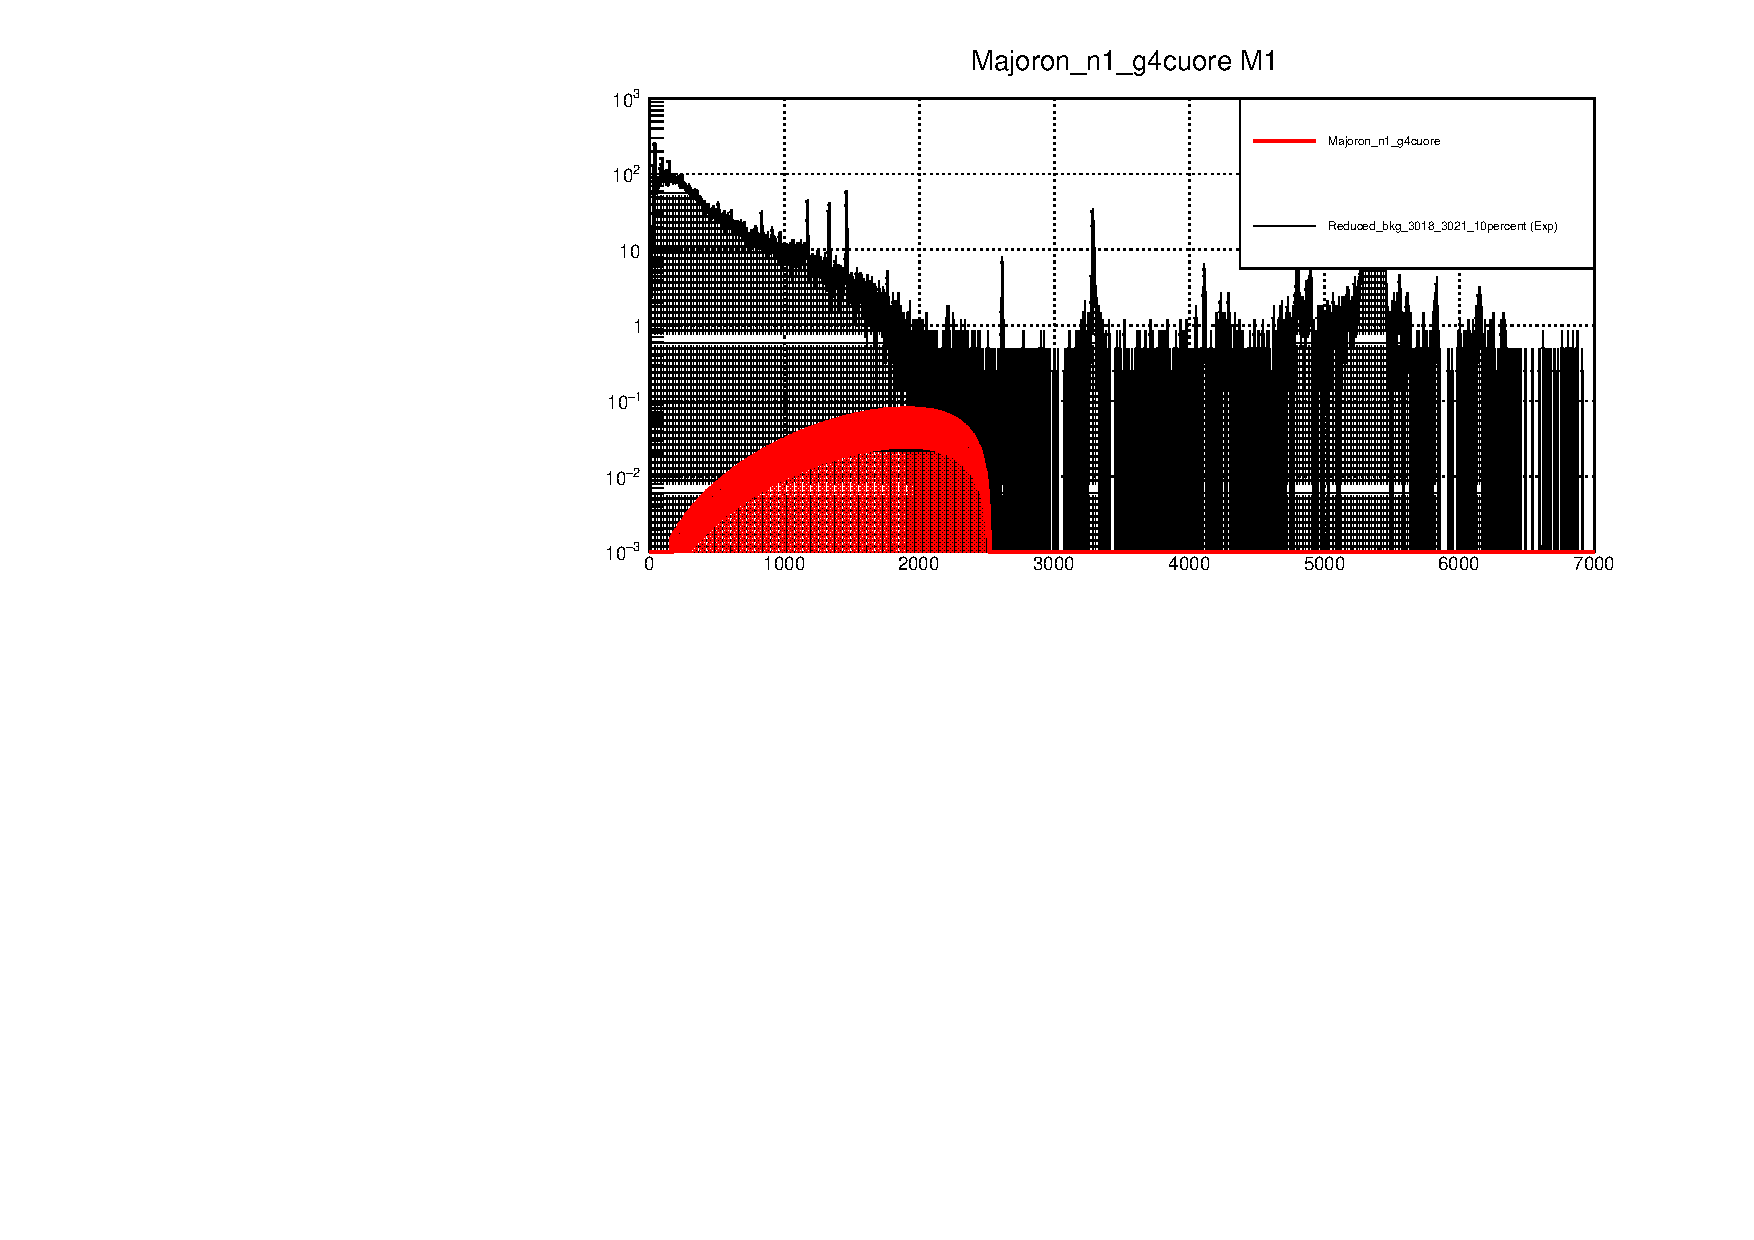
\includegraphics[width=0.9\textwidth]{Figures/Majoron_n1_g4cuore.pdf}
\end{subfigure}
\qquad
\begin{subfigure}[t]{0.49\textwidth}
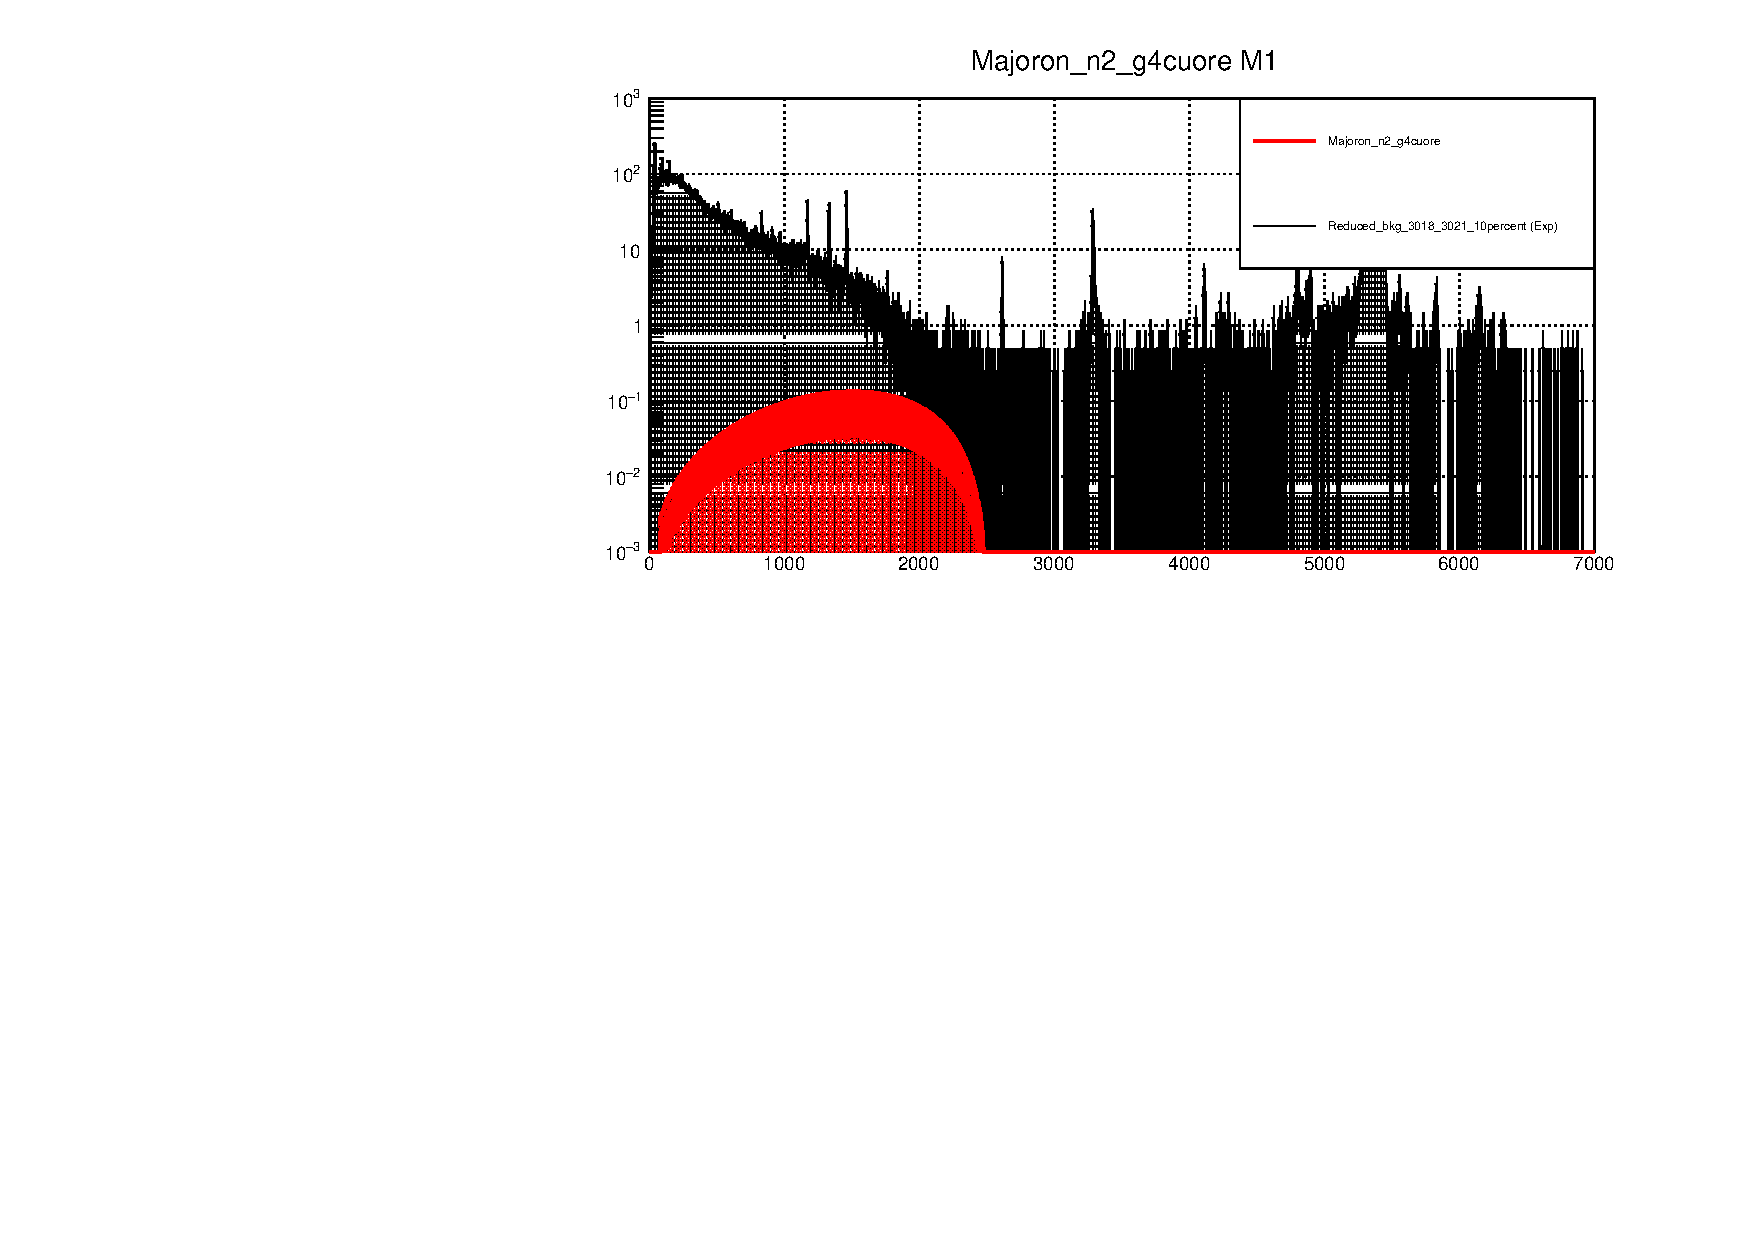
\includegraphics[width=0.9\textwidth]{Figures/Majoron_n2_g4cuore.pdf}
\end{subfigure}
\qquad
\begin{subfigure}[t]{0.49\linewidth}
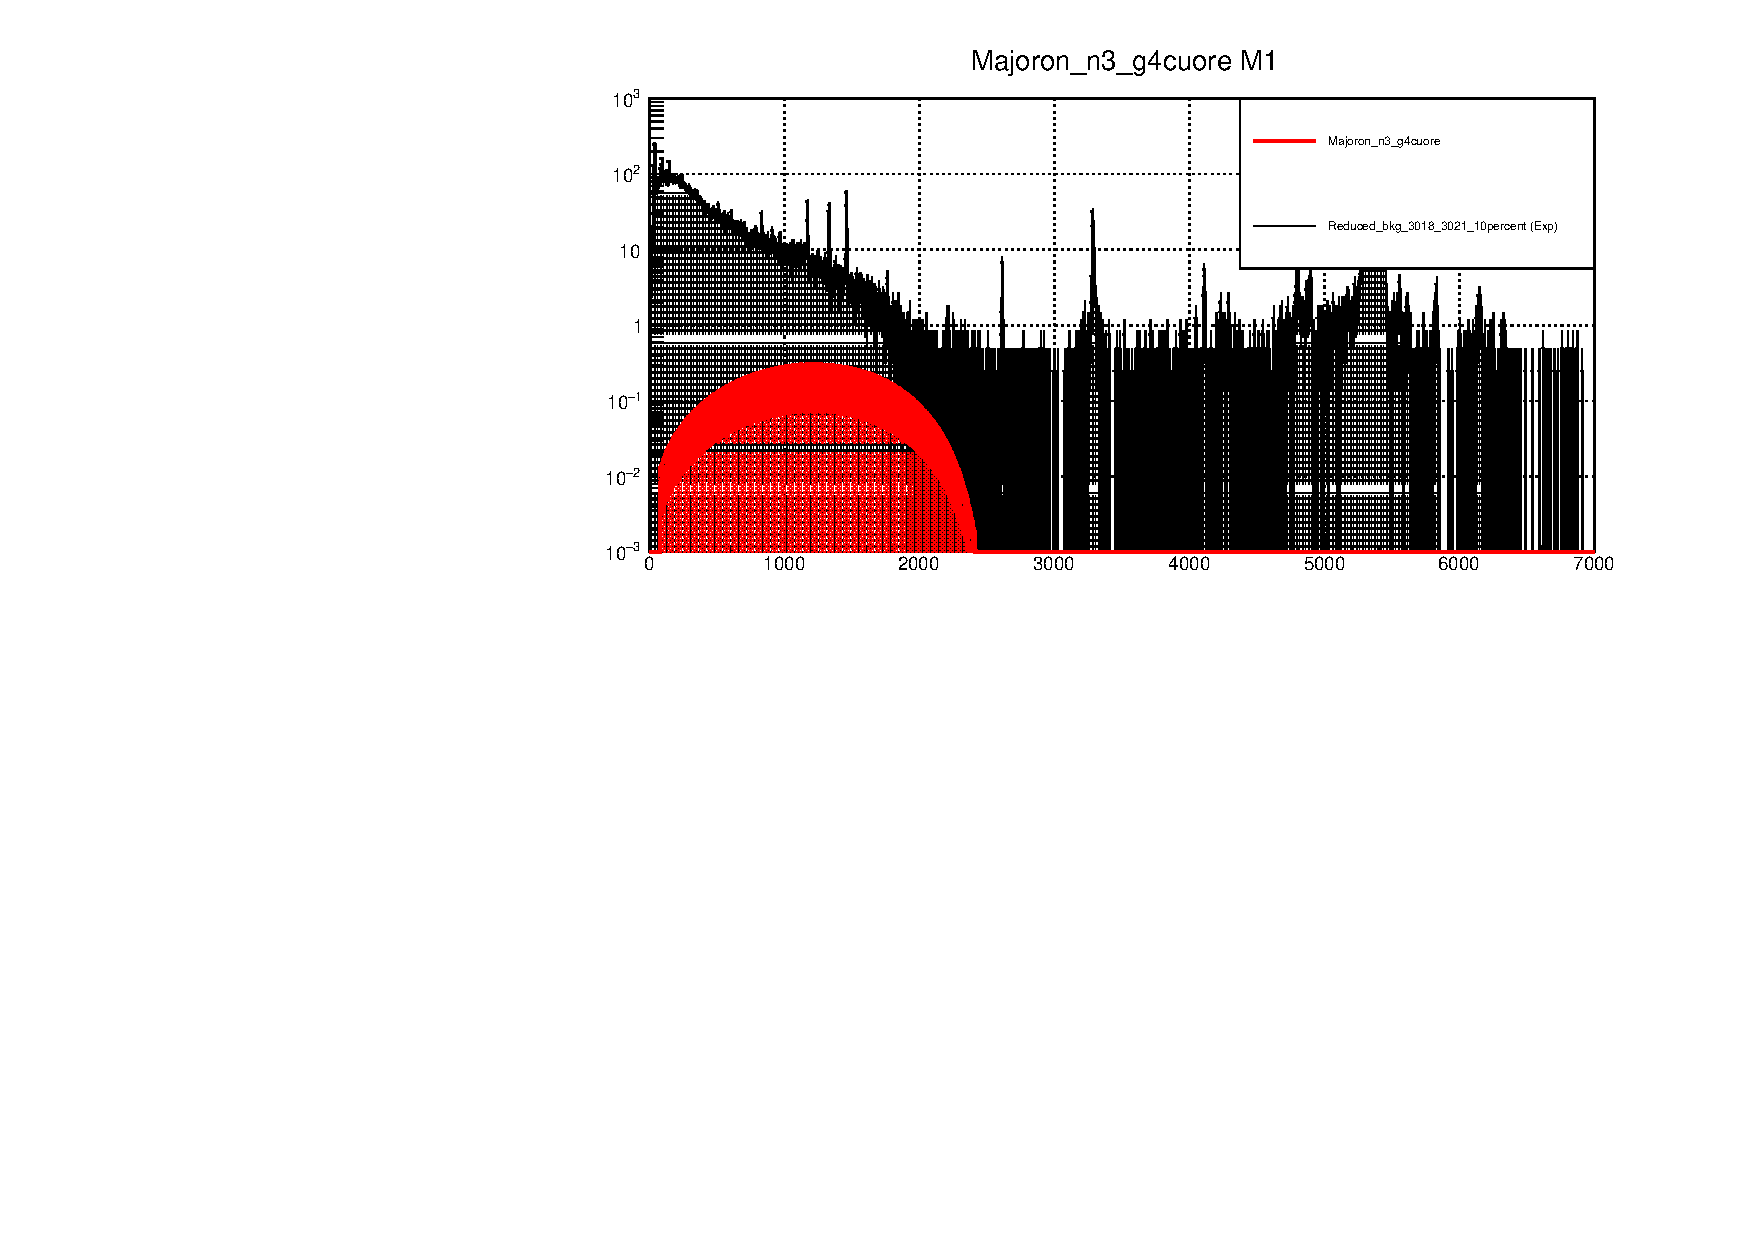
\includegraphics[width=0.9\textwidth]{Figures/Majoron_n3_g4cuore.pdf}
\end{subfigure}
\qquad
\begin{subfigure}[t]{0.49\linewidth}
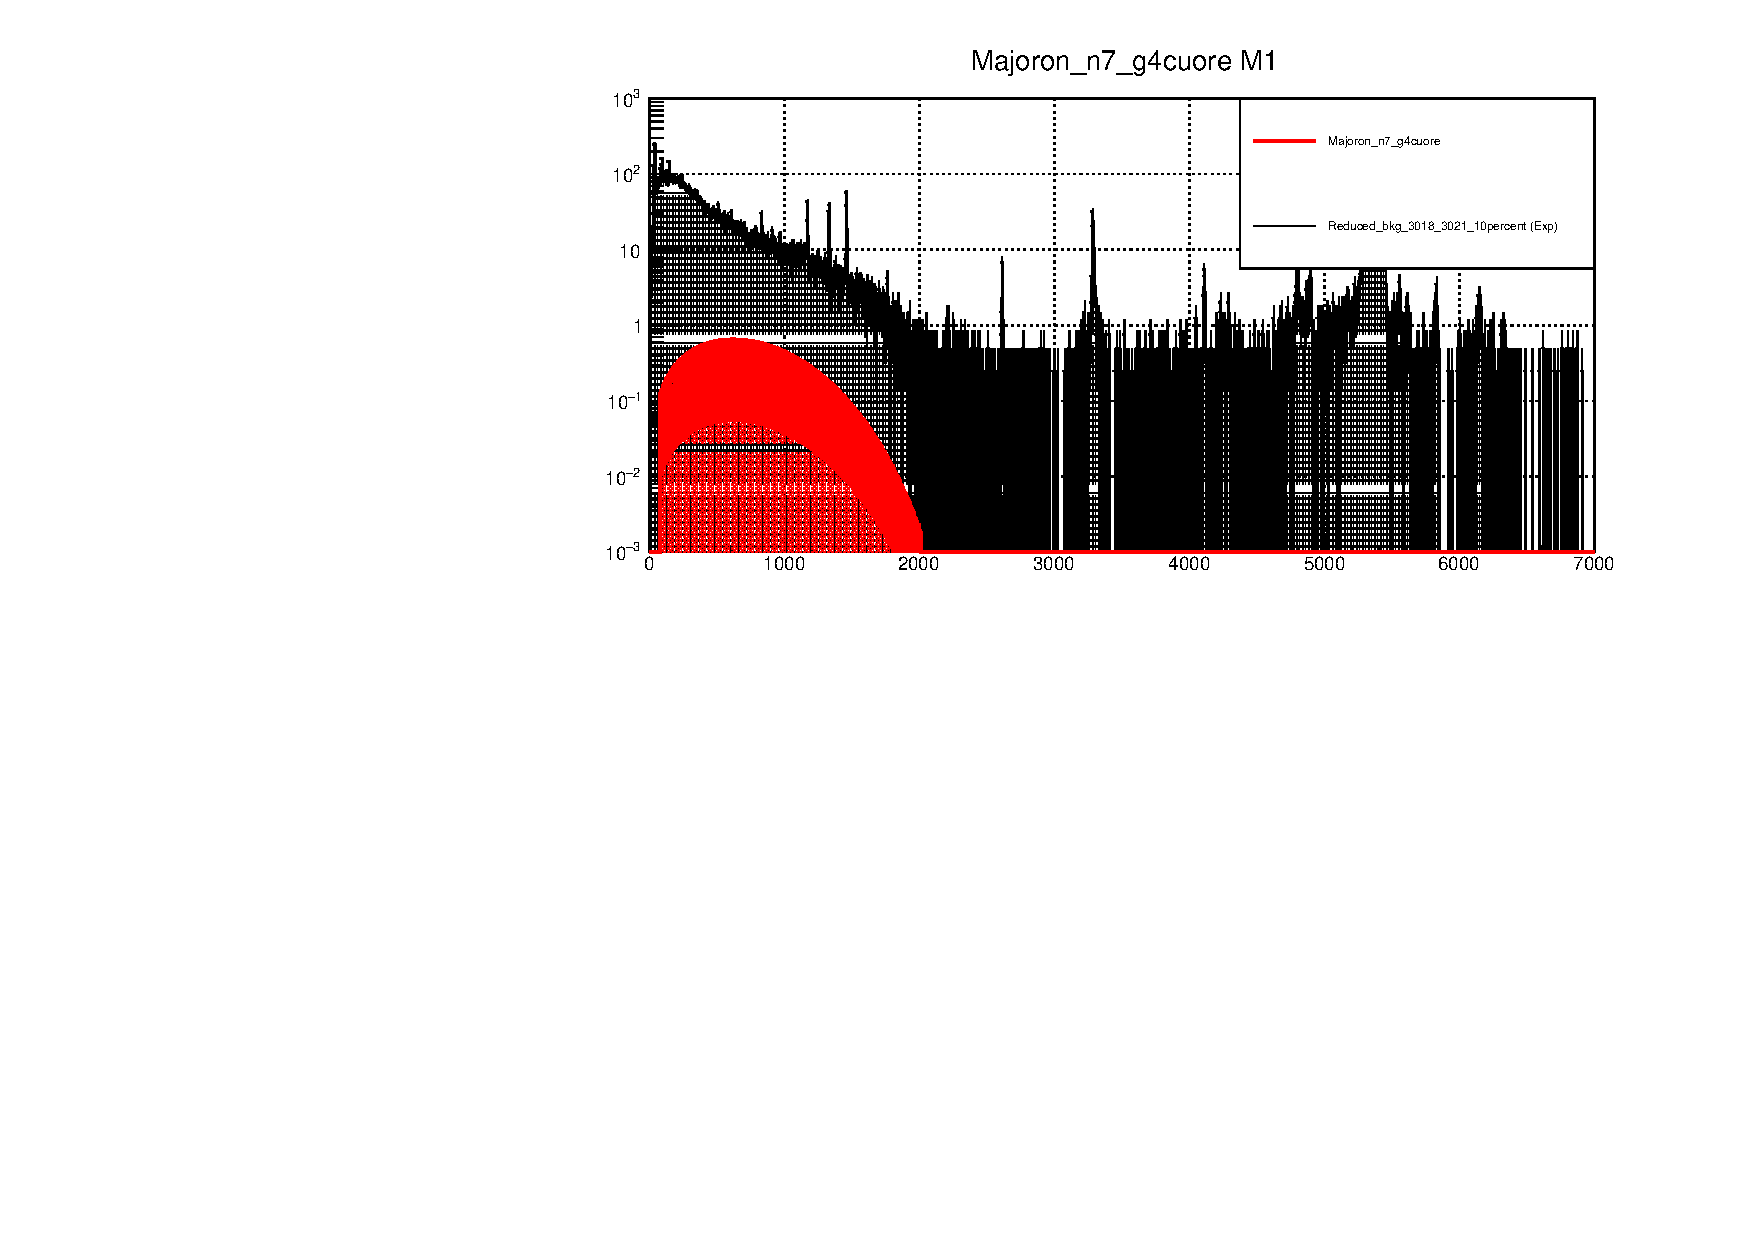
\includegraphics[width=0.9\textwidth]{Figures/Majoron_n7_g4cuore.pdf}
\end{subfigure}
\caption[The fitted contribution of Majoron decays for the different spectral indices in the \Mone~ spectrum.]{The fitted contribution of Majoron decays for the different spectral indices in the \Mone~ spectrum.}
\label{fig:SpectralIndicesM1Fit}
\end{figure}

\begin{figure}[htbp]
\centering
\begin{subfigure}[t]{0.49\textwidth}
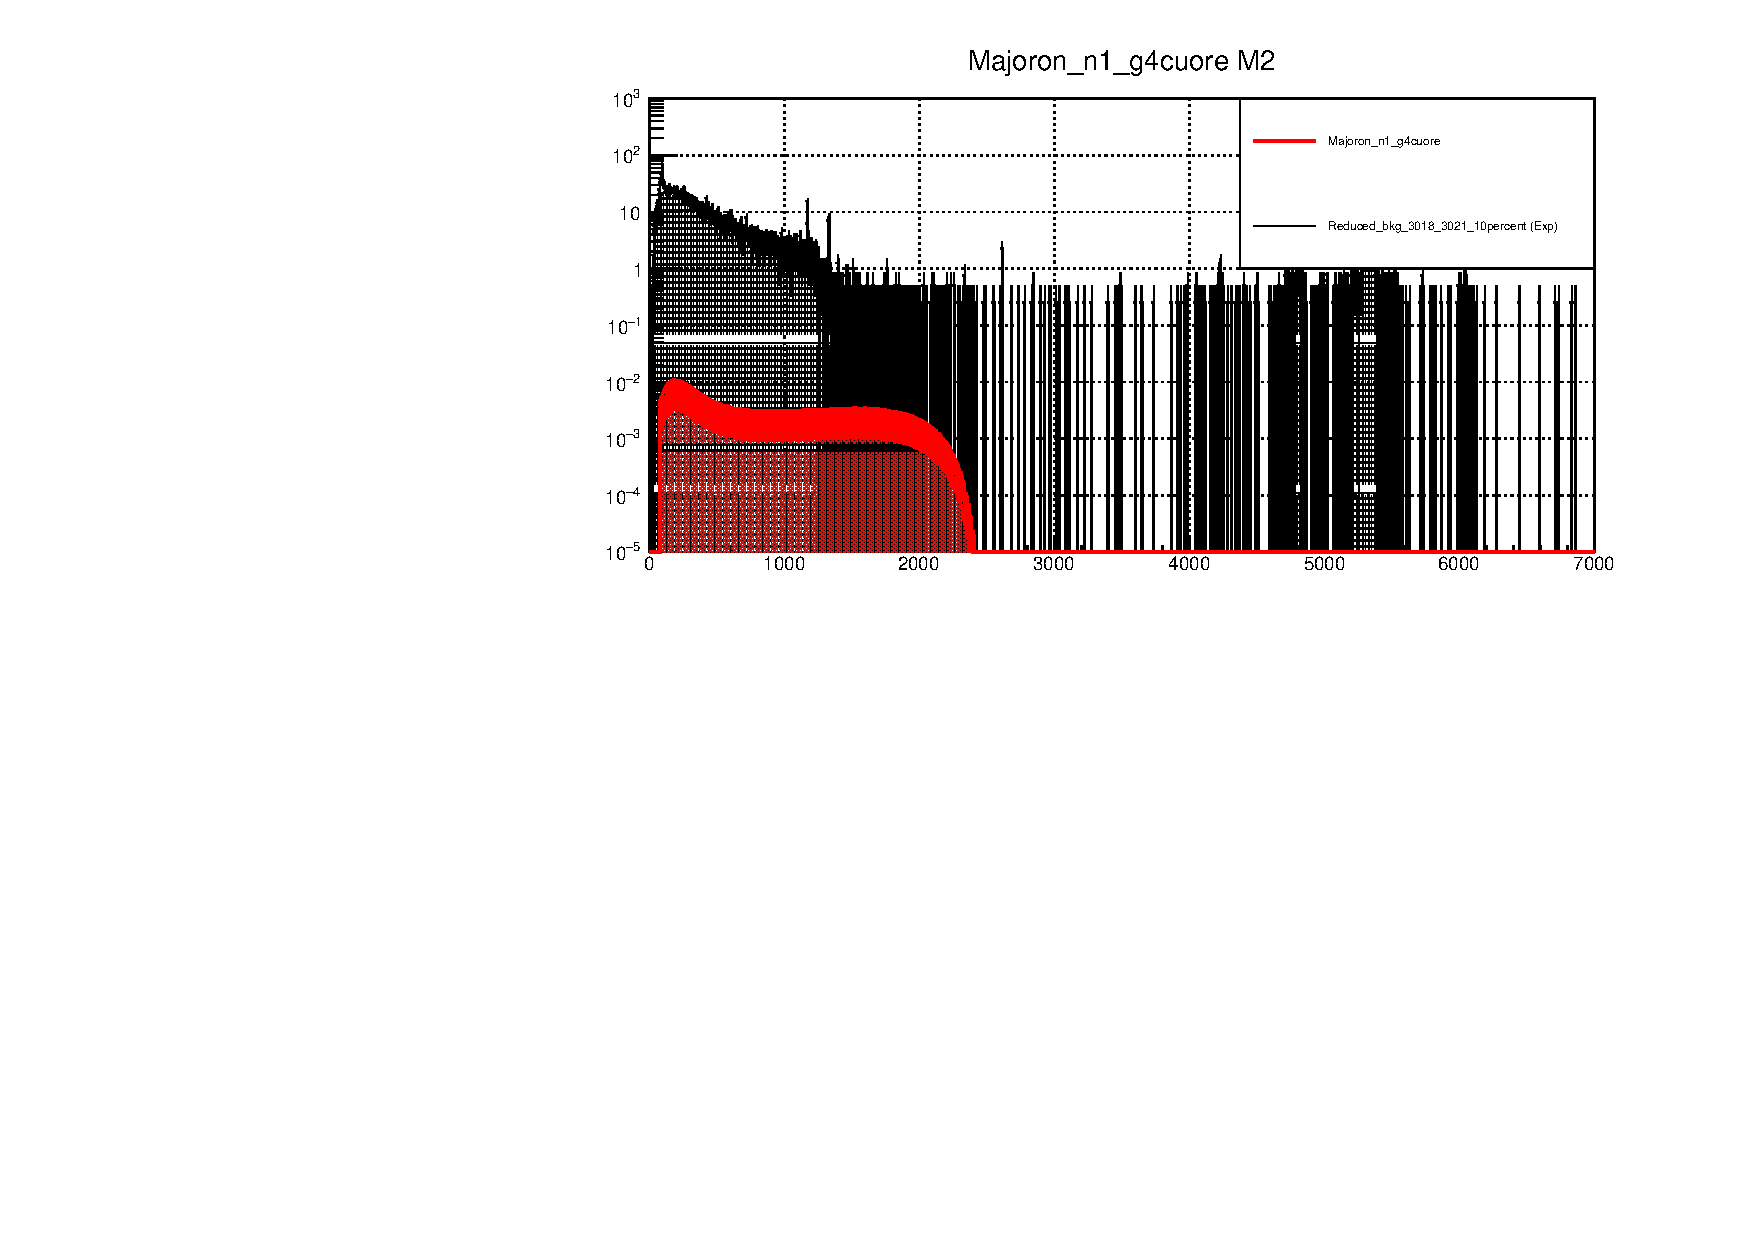
\includegraphics[width=0.9\textwidth]{Figures/Majoron_n1_g4cuore_M2.pdf}
\end{subfigure}
\qquad
\begin{subfigure}[t]{0.49\textwidth}
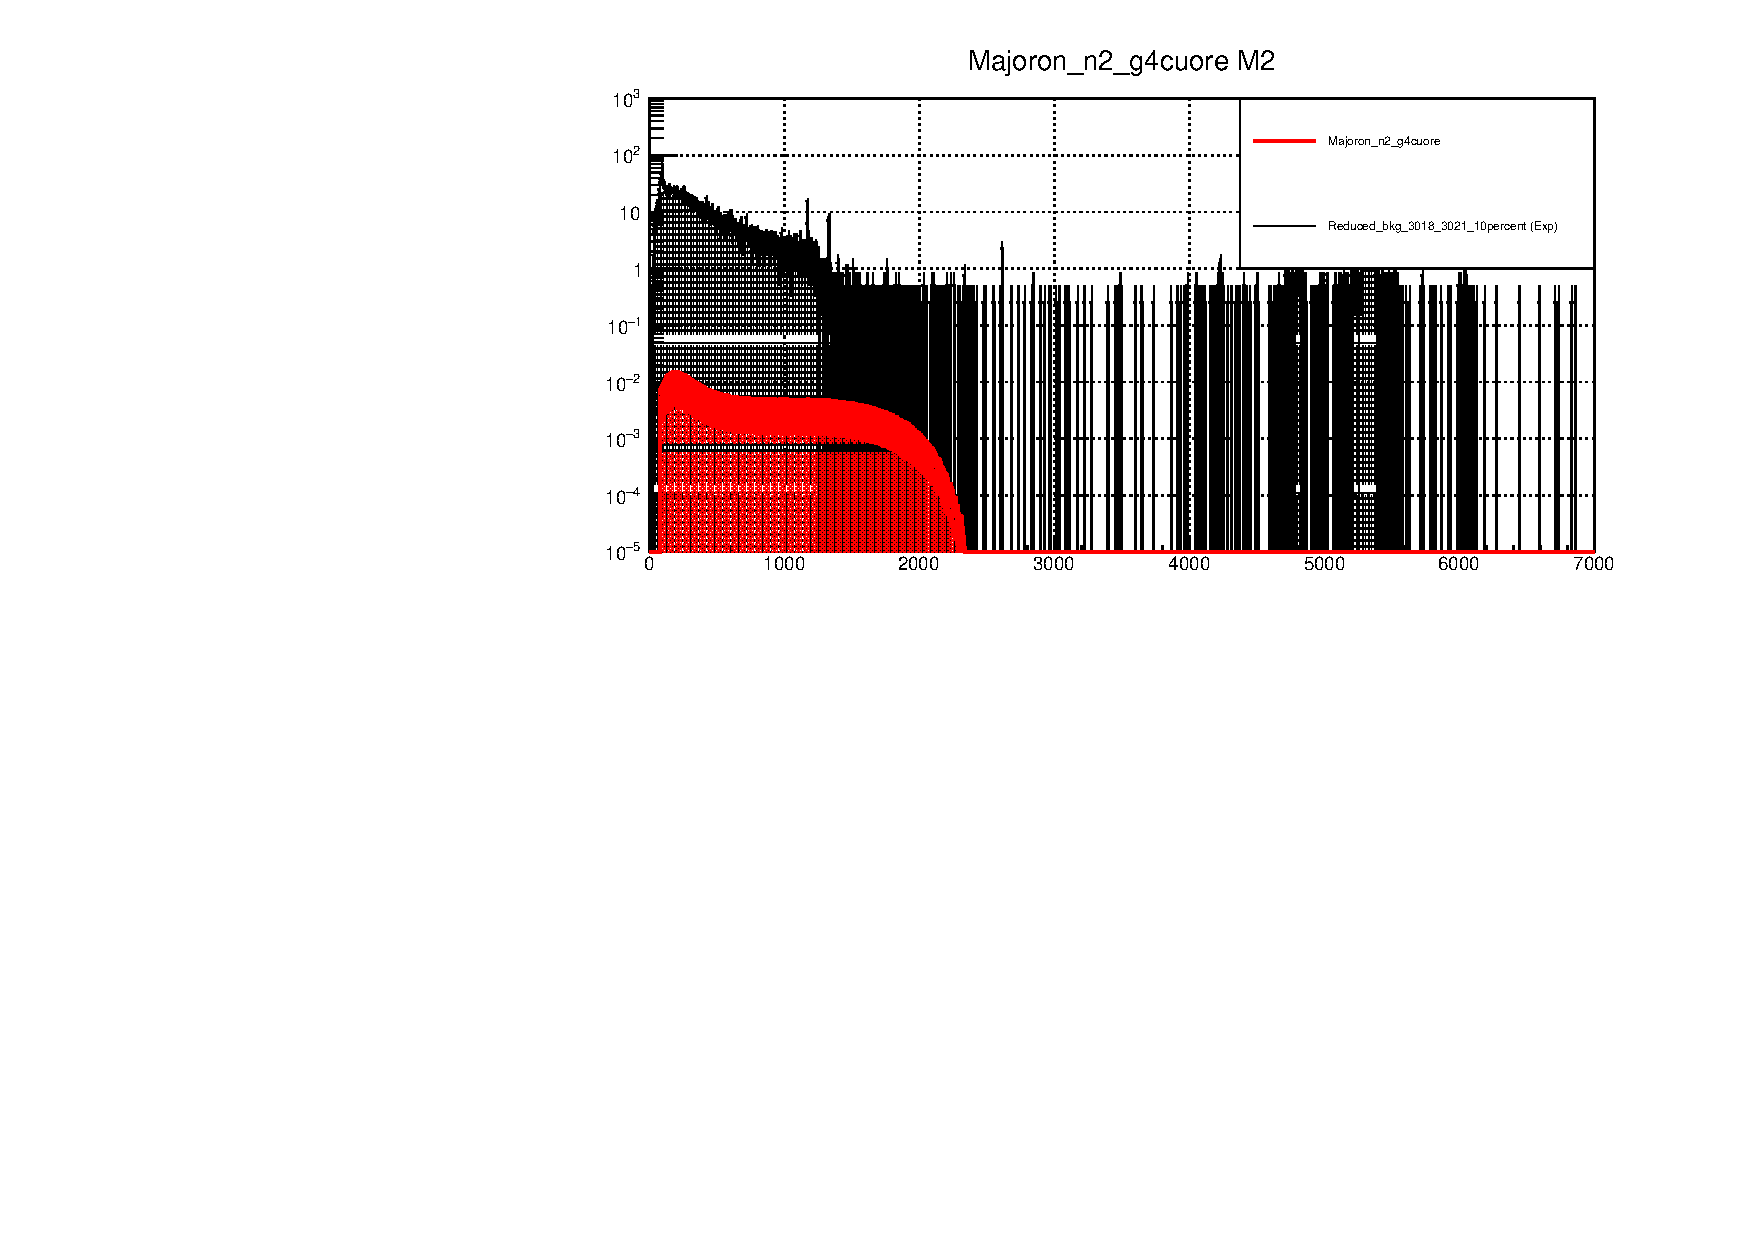
\includegraphics[width=0.9\textwidth]{Figures/Majoron_n2_g4cuore_M2.pdf}
\end{subfigure}
\qquad
\begin{subfigure}[t]{0.49\linewidth}
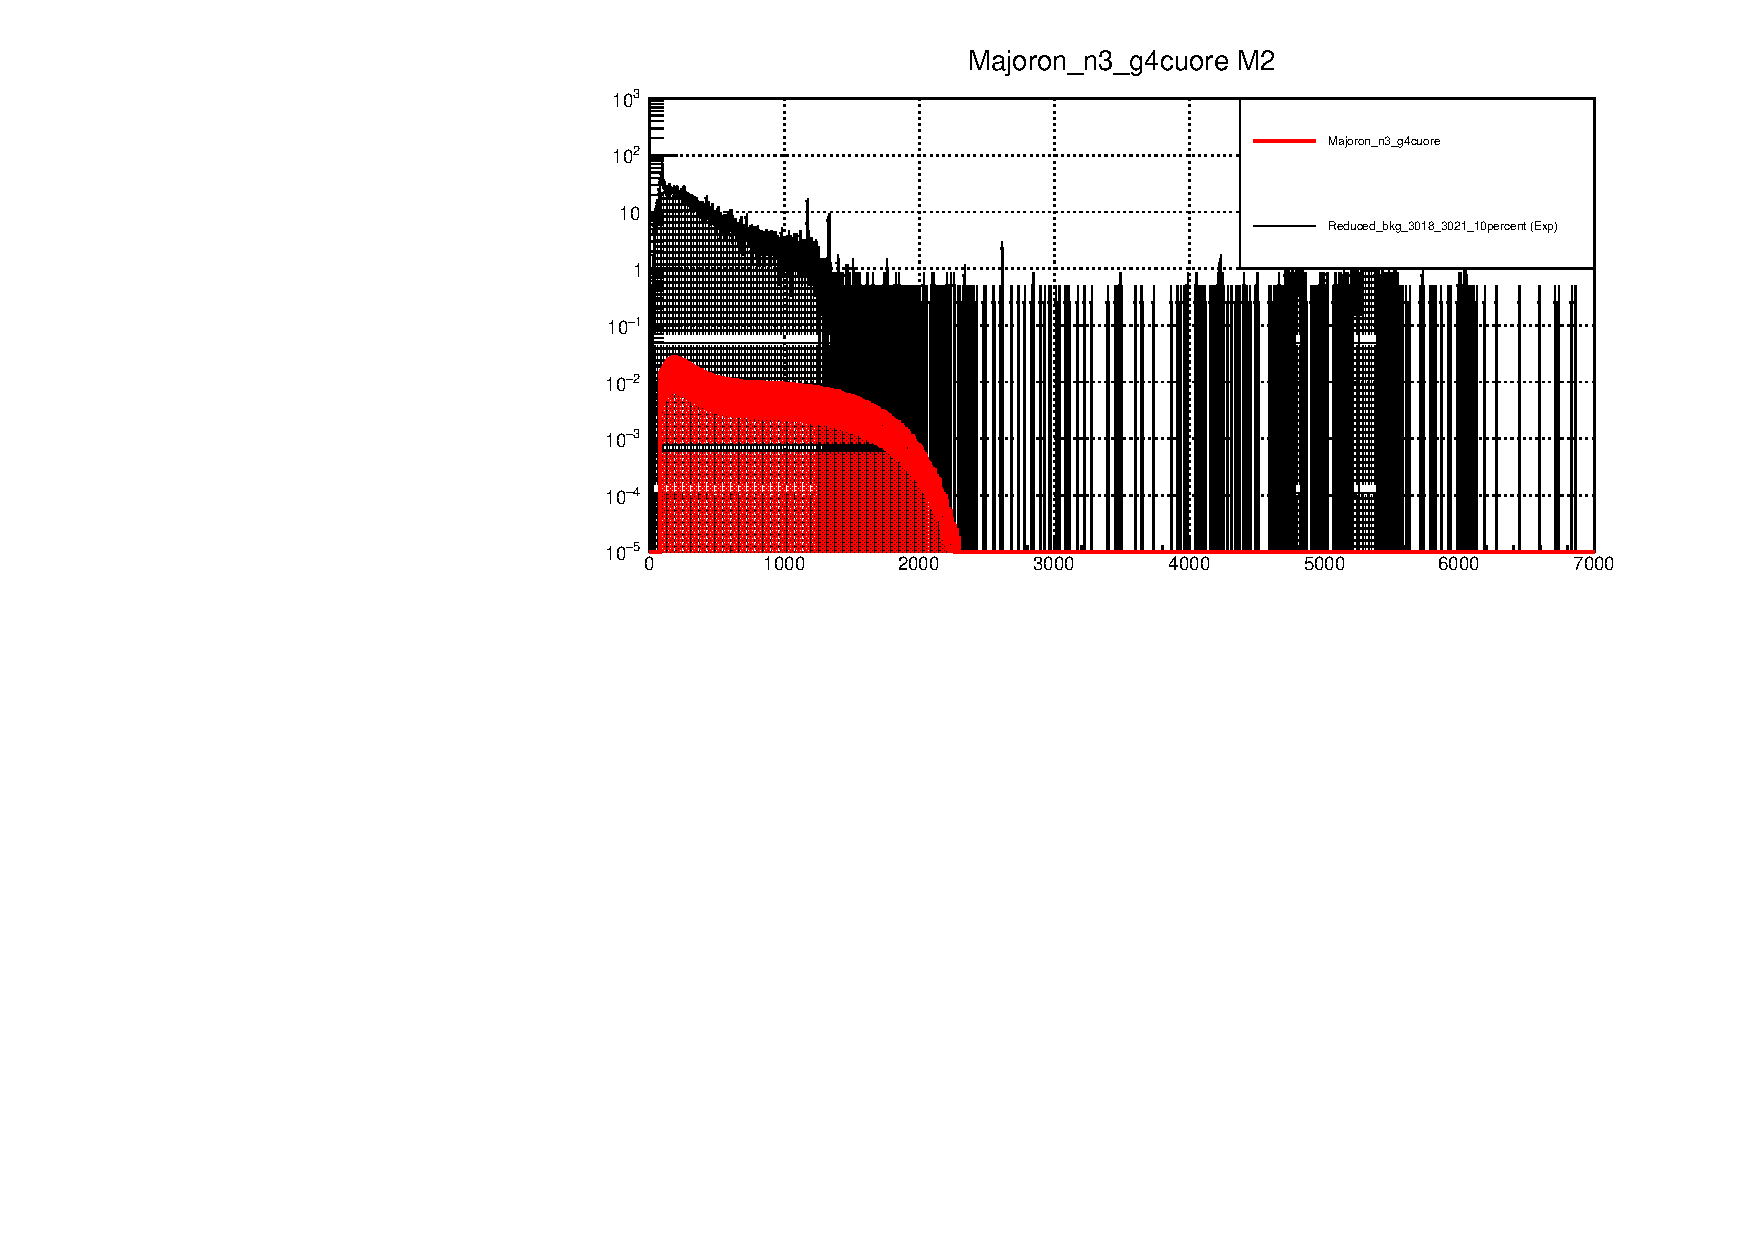
\includegraphics[width=0.9\textwidth]{Figures/Majoron_n3_g4cuore_M2.pdf}
\end{subfigure}
\qquad
\begin{subfigure}[t]{0.49\linewidth}
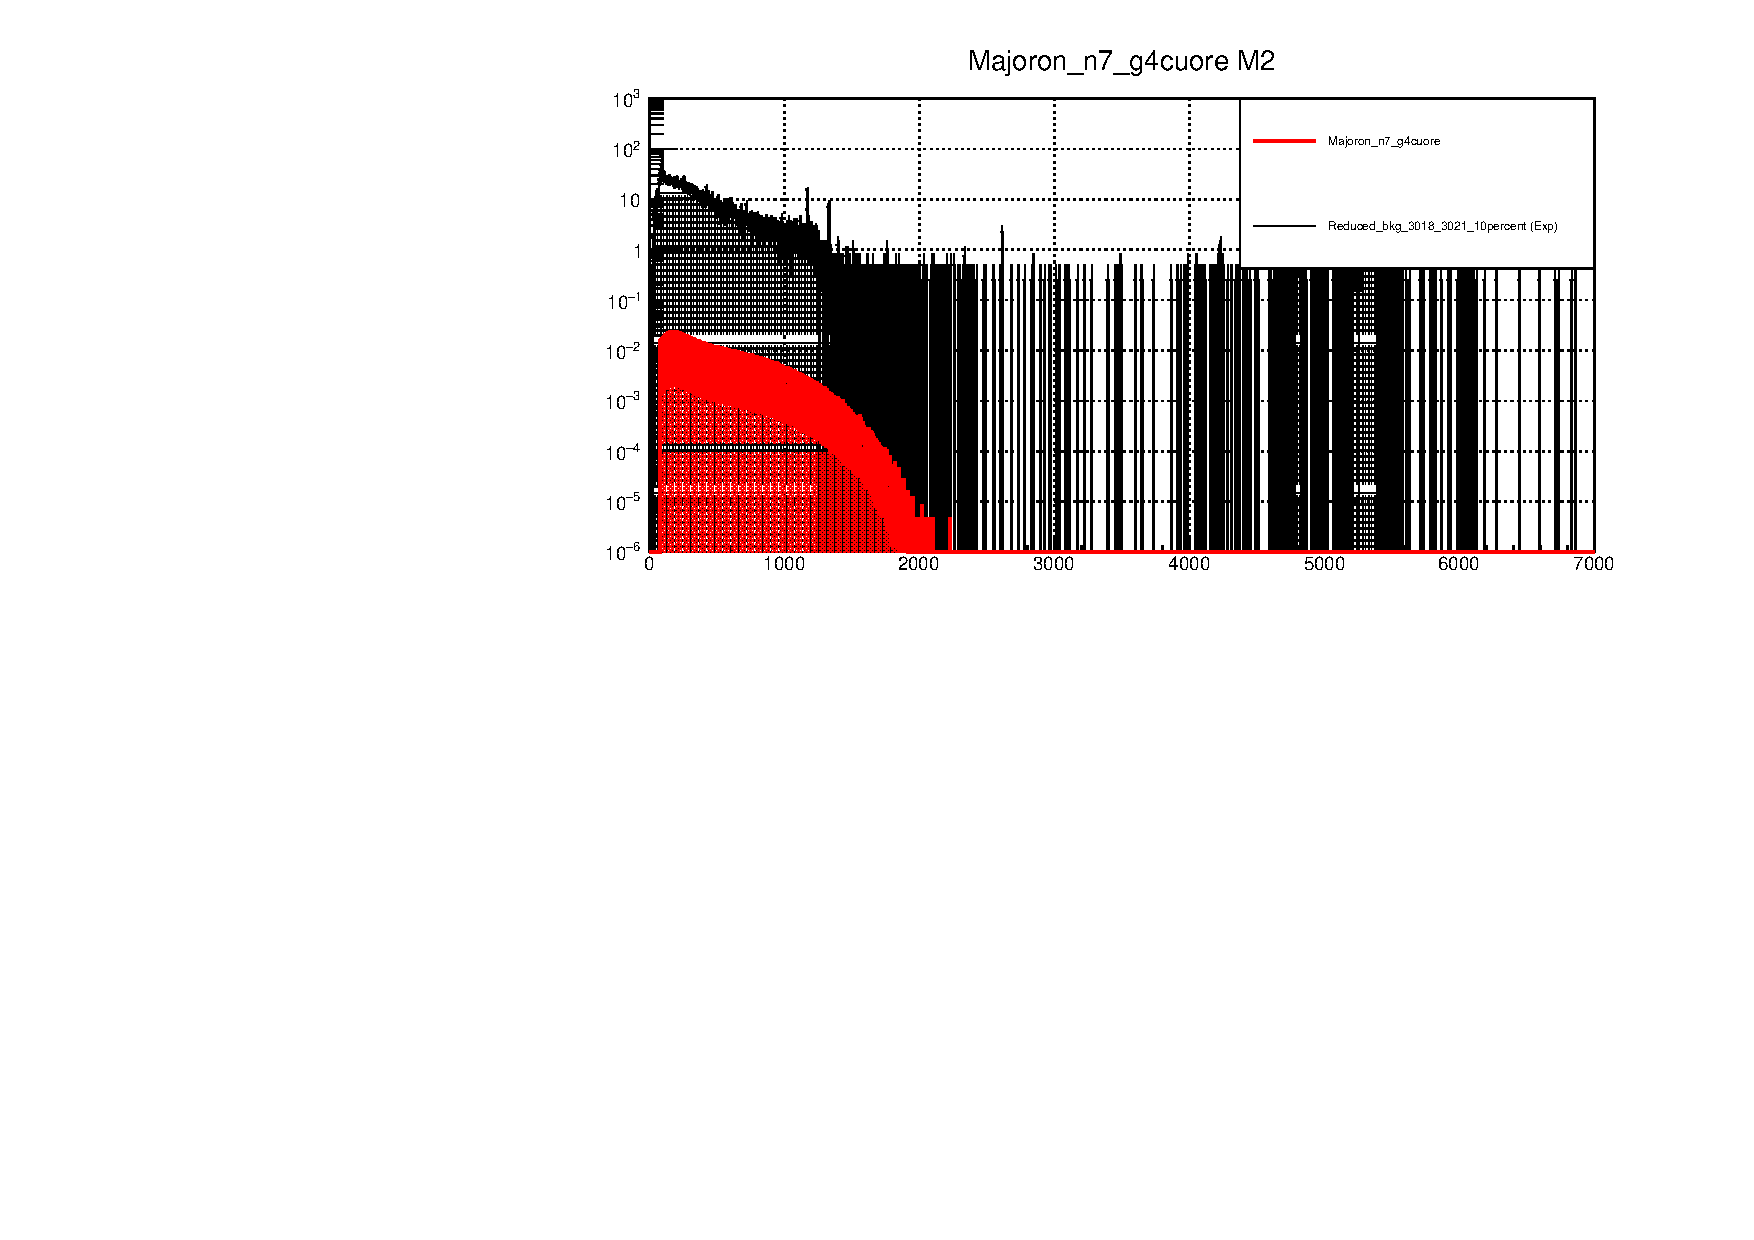
\includegraphics[width=0.9\textwidth]{Figures/Majoron_n7_g4cuore_M2.pdf}
\end{subfigure}
\caption[The fitted contribution of Majoron decays for the different spectral indices in the \Mtwo~ spectrum.]{The fitted contribution of Majoron decays for the different spectral indices in the \Mtwo~ spectrum.}
\label{fig:SpectralIndicesM2Fit}
\end{figure}

Figures to include: Correlation matrix, Fit value distributions for all the Majoron spectra, background model with only 2nu -- describe deficiencies i.e. alpha region low-E and 2 MeV, systematics (floors, layers, etc.), 

\section{Majoron Systematics}